\documentclass[10pt, aspectratio=169, handout]{beamer}
\usefonttheme{professionalfonts}
%\usetheme{CambridgeUS}
%
% Choose how your presentation looks.
%
% For more themes, color themes and font themes, see:
% http://deic.uab.es/~iblanes/beamer_gallery/index_by_theme.html
%
\mode<presentation>
{
  \usetheme{Berkeley}      % or try Darmstadt, Madrid, Warsaw, ...
  \usecolortheme{beaver} % or try albatross, beaver, crane, ...
  \usefonttheme{default}  % or try serif, structurebold, ...
  \setbeamertemplate{navigation symbols}{}
  \setbeamertemplate{caption}[numbered]
} 

\setbeamertemplate{footline}{%
  \leavevmode%
  \hbox{%
    \begin{beamercolorbox}[wd=.85\paperwidth,ht=2.5ex,dp=1ex,left]{author in head/foot}%
      \usebeamerfont{author in head/foot}Maxx Seminario, Electronic Circuits, Fall 2025%
    \end{beamercolorbox}%
    \begin{beamercolorbox}[wd=.15\paperwidth,ht=2.5ex,dp=1ex,right]{date in head/foot}%
      \hspace*{0.5em}\insertframenumber{} / \inserttotalframenumber\hspace*{0.5em}%
    \end{beamercolorbox}%
  }%
  \vskip0pt%
}

\usepackage[english]{babel}
\usepackage[utf8x]{inputenc}
\usepackage{tikz}
\usepackage{pgfplots}
\usepackage{array}  % for table column M
\usepackage{makecell} % to break line within a cell
\usepackage{verbatim}
\usepackage{graphicx}
\usepackage{subcaption}
\usepackage{amsfonts}
\usepackage{amsmath}
\usepackage{bm}
\usepackage{epstopdf}
\usepackage{circuitikz}
\usepackage{caption}
\captionsetup{compatibility=false}
%\usepackage{dsfont}
\usepackage[absolute,overlay]{textpos}
\usetikzlibrary{calc}
\usetikzlibrary{pgfplots.fillbetween, backgrounds}
\usetikzlibrary{positioning}

\usetikzlibrary{pgfplots.groupplots}
\usetikzlibrary{plotmarks}
\usetikzlibrary{calc}

\usepgfplotslibrary{groupplots}
\pgfplotsset{compat=newest} 
%\pgfplotsset{plot coordinates/math parser=false}

\usepackage{hyperref}
\hypersetup{
    colorlinks=true,
    linkcolor=blue,
    filecolor=magenta,      
    urlcolor=cyan,
}

% %% 
% \input{header.tex}

% %%
\title[ECEN 463/863]{Electronic Signals}
\author{Maxx Seminario}
\institute{University of Nebraska-Lincoln}
\date{January 2025}

\begin{document}
\begin{frame}
  \titlepage
\end{frame}

\section{What are Signals?}

\begin{frame}{Signals: Information Carriers}
    
    \textbf{Definition}:  Signals contain information about physical phenomena
    
    \vspace{0.3cm}
    
    \begin{columns}[b]
    \column{0.3\textwidth}
        \textbf{Weather}:
        \begin{itemize}
            \item Temperature
            \item Pressure
            \item Humidity
        \end{itemize}
        
        \begin{figure}[b]
        \centering
        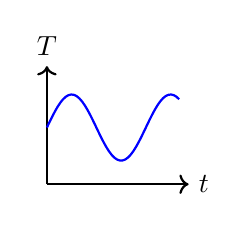
\begin{tikzpicture}[scale=0.6]
            \draw[->, thick] (0,0) -- (3,0) node[right] {$t$};
            \draw[->, thick] (0,0) -- (0,2.5) node[above] {$T$};
            \draw[blue, thick, domain=0:2.8, samples=50] plot (\x, {1.2 + 0.7*sin(3*\x r)});
        \end{tikzpicture}
        \end{figure}
        
    \column{0.3\textwidth}
        \textbf{Audio}:
        \begin{itemize}
            \item Voice
            \item Music
            \item Environmental sounds
        \end{itemize}
        
        \begin{figure}[b]
        \centering
        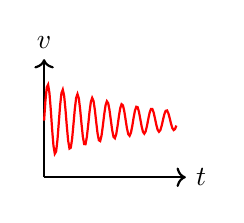
\begin{tikzpicture}[scale=0.6]
            \draw[->, thick] (0,0) -- (3,0) node[right] {$t$};
            \draw[->, thick] (0,0) -- (0,2.5) node[above] {$v$};
            \draw[red, thick, domain=0:2.8, samples=100] plot (\x, {1.2 + 0.8*sin(20*\x r)*exp(-0.5*\x)});
        \end{tikzpicture}
        \end{figure}
        
    \column{0.3\textwidth}
        \textbf{Industrial}:
        \begin{itemize}
            \item Machine status
            \item Process control
            \item Safety monitoring
        \end{itemize}
        
        \begin{figure}[htb]
        \centering
        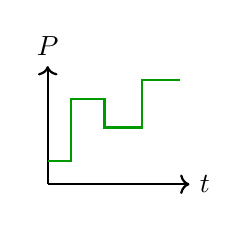
\begin{tikzpicture}[scale=0.6]
            \draw[->, thick] (0,0) -- (3,0) node[right] {$t$};
            \draw[->, thick] (0,0) -- (0,2.5) node[above] {$P$};
            \draw[green! 60! black, thick] plot coordinates {(0,0.5) (0.5,0.5) (0.5,1.8) (1.2,1.8) (1.2,1.2) (2,1.2) (2,2.2) (2.8,2.2)};
        \end{tikzpicture}
        \end{figure}
        
    \end{columns}
    
    \vspace{0.4cm}
    
    \begin{block}{The Challenge}
        How do we extract useful information from these signals?
    \end{block}
    
\end{frame}

\begin{frame}{From Physical to Electrical Signals}
    
    \begin{columns}[t]
    \column{0.48\textwidth}
        \textbf{The Transducer}:
        \begin{itemize}
            \item Converts physical signals to electrical
            \item Output: voltage or current
            \item Many types for different phenomena
        \end{itemize}
        
        \vspace{0.3cm}
        
        \textbf{Examples}:
        \begin{itemize}
            \item Microphone: sound $\rightarrow$ voltage
            \item Thermistor: temperature $\rightarrow$ resistance
            \item Photodiode: light $\rightarrow$ current
            \item Accelerometer: motion $\rightarrow$ voltage
        \end{itemize}
        
    \column{0.48\textwidth}
        \begin{figure}[htb]
        \centering
        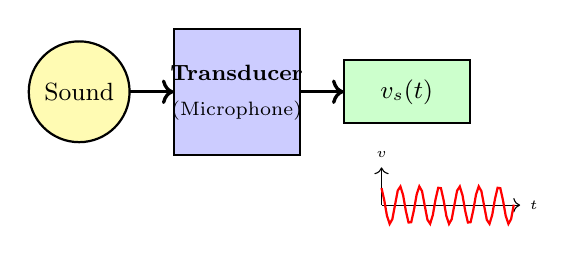
\begin{tikzpicture}[scale=0.8]
            % Physical signal
            \draw[fill=yellow!30, thick] (0,2) circle (0.8);
            \node at (0,2) {\small Sound};
            \draw[->, very thick] (0.8,2) -- (1.5,2);
            
            % Rectangle
            \draw[fill=blue!20, thick] (1.5,1) rectangle (3.5,3);

            % Labels with smaller fonts
            \node[font=\footnotesize\bfseries] at (2.5,2.3) {Transducer};
            \node[font=\scriptsize] at (2.5,1.7) {(Microphone)};

            % Electrical signal
            \draw[->, very thick] (3.5,2) -- (4.2,2);
            \draw[fill=green!20, thick] (4.2,1.5) rectangle (6.2,2.5);
            \node at (5.2,2) {\small $v_s(t)$};
            
            % Waveform
            \begin{scope}[shift={(2.5,0.2)}]
                \draw[->, thin] (2.3,0) -- (4.5,0) node[right] {\tiny $t$};
                \draw[->, thin] (2.3,0) -- (2.3,0.6) node[above] {\tiny $v$};
                \draw[red, thick, domain=2.3:4.4, samples=50] plot (\x, {0.3*sin(20*\x r)});
            \end{scope}
        \end{tikzpicture}
        \caption{Transducer converts physical signal to electrical}
        \end{figure}
        
    \end{columns}
    
    \vspace{0.3cm}
    
    \begin{block}{Assumption in This Course}
        Signals already exist in the electrical domain (voltage or current)
    \end{block}
    
\end{frame}

\section{Signal Source Representations}

\begin{frame}{Thevenin and Norton Representations}
    
    \begin{columns}[t]
    \column{0.48\textwidth}
        \textbf{Thevenin Form}:
        \begin{itemize}
            \item Voltage source $v_s(t)$
            \item Series resistance $R_s$
            % \item Preferred when $R_s$ is \textbf{low}
        \end{itemize}
        
        % \vspace{0.3cm}
        
        \begin{figure}[b]
        \centering
        \begin{circuitikz}[scale=1.0]
            \draw (0,0) to[sV, l=$v_s(t)$] (0,2);
            \draw (0,2) to[R, l=$R_s$] (2,2);
            \draw (0,0) -- (2,0);
            \draw (2,0) to[open, v^>=$v_{oc}$] (2,2);
            \draw[fill=black] (2,2) circle (0.05);
            \draw[fill=black] (2,0) circle (0.05);
        \end{circuitikz}
        \caption{Thevenin equivalent circuit}
        \end{figure}
        
    \column{0.48\textwidth}
        \textbf{Norton Form}:
        \begin{itemize}
            \item Current source $i_s(t)$
            \item Parallel resistance $R_s$
            % \item Preferred when $R_s$ is \textbf{high}
        \end{itemize}
        
        % \vspace{0.3cm}
        
        \begin{figure}[b]
        \centering
        \begin{circuitikz}[scale=1.0]
            \draw (0,0) to[sI, l=$i_s(t)$] (0,2);
            \draw (0,2) to[short] (1,2);
            \draw (1,2) to[R, l=$R_s$] (1,0);
            \draw (1,0) to[short] (0,0);
            \draw (1,0) to[short] (2,0);
            \draw (1,2) to[short] (2,2);
            \draw[fill=black] (2,2) circle (0.05);
            \draw[fill=black] (2,0) circle (0.05);
        \end{circuitikz}
        \caption{Norton equivalent circuit}
        \end{figure}
        
    \end{columns}
    
    % \vspace{0.3cm}
    
    \begin{block}{Equivalence Condition}
        % For the two representations to be equivalent: 
        $v_s(t) = R_s \cdot i_s(t)$  For the two representations to be equivalent
        
    \end{block}
    
\end{frame}

\begin{frame}{Source Resistance:  The Imperfection}
    
    \begin{columns}[t]
    \column{0.48\textwidth}
        \textbf{Thevenin Source with Load}:
        
        \begin{figure}[t]
        \centering
        \begin{circuitikz}[scale=0.8]
            \draw (0,0) to[sV, l=$v_s$] (0,2.5);
            \draw (0,2.5) to[R, l=$R_s$] (2.5,2.5);
            \draw (2.5,2.5) to[R, l=$R_L$, v_>=$v_o$] (2.5,0);
            \draw (2.5,0) -- (0,0);
        \end{circuitikz}
        \end{figure}
        
        \vspace{0.2cm}
        
        \textbf{Voltage divider}: $v_o = v_s \frac{R_L}{R_L + R_s}$

        \vspace{0.2cm}
        
        \textbf{Condition for} $v_o \approx v_s$: $\boxed{R_s \ll R_L}$
        
    \column{0.48\textwidth}
        \textbf{Norton Source with Load}:
        
        \begin{figure}[t]
        \centering
        \begin{circuitikz}[scale=0.8]
            \draw (0,0) to[sI, l=$i_s$] (0,2.5);
            \draw (0,2.5) -- (1.25,2.5);
            \draw (1.25,2.5) to[R, l=$R_s$] (1.25,0);
            \draw (1.25,2.5) -- (2.5,2.5);
            \draw (2.5,2.5) to[R, l=$R_L$, i>^=$i_o$] (2.5,0);
            \draw (0,0) -- (2.5,0);
        \end{circuitikz}
        \end{figure}
        
        \vspace{1.0cm}
        
        \textbf{Current divider}: $i_o = i_s \frac{R_s}{R_s + R_L}$

        \vspace{0.2cm}
        
        \textbf{Condition for} $i_o \approx i_s$: $\boxed{R_s \gg R_L}$
        
    \end{columns}
    
    % \vspace{0.3cm}
    
    \begin{alertblock}{Important}
        Source resistance $R_s$ limits signal delivery to the load! 
    \end{alertblock}
    
\end{frame}

\begin{frame}{Signal Loss Due to Source Resistance}
    
    \begin{figure}[htb]
    \centering
    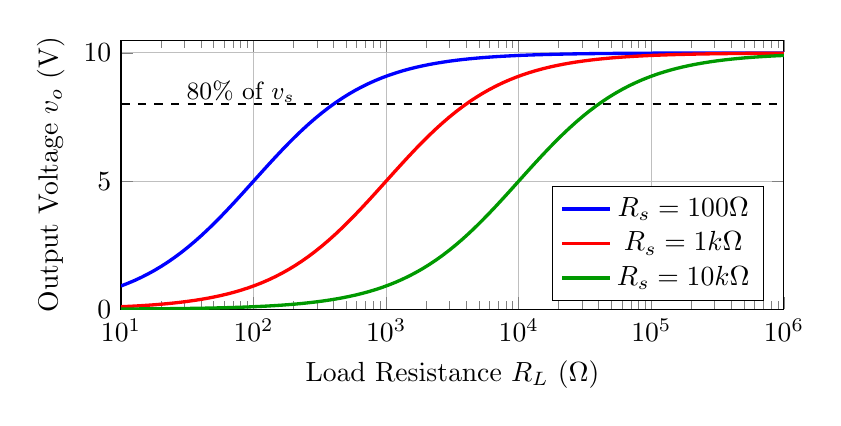
\begin{tikzpicture}
        \begin{axis}[
            width=10cm, height=5cm,
            xlabel={Load Resistance $R_L$ ($\Omega$)},
            ylabel={Output Voltage $v_o$ (V)},
            xmode=log,
            domain=10: 1000000,
            samples=100,
            grid=major,
            legend pos=south east,
            xmin=10, xmax=1000000,
            ymin=0, ymax=10.5,
        ]
        
        % Rs = 100 ohm, vs = 10V
        \addplot[blue, very thick] {10*x/(x+100)};
        \addlegendentry{$R_s = 100 \Omega$}
        
        % Rs = 1k ohm, vs = 10V
        \addplot[red, very thick] {10*x/(x+1000)};
        \addlegendentry{$R_s = 1k \Omega$}
        
        % Rs = 10k ohm, vs = 10V
        \addplot[green!60!black, very thick] {10*x/(x+10000)};
        \addlegendentry{$R_s = 10k \Omega$}
        
        % 80% line
        \addplot[dashed, thick, black] coordinates {(1,8) (1000000,8)};
        \node at (axis cs:80,8.5) {\small 80\% of $v_s$};
        
        \end{axis}
    \end{tikzpicture}
    \caption{Thevenin source:  output voltage vs. load resistance ($v_s = 10 V$)}
    \end{figure}
    
    \vspace{-0.5cm}
    
    \begin{block}{Design Insight}
        Higher $R_s$ requires higher $R_L$ to minimize signal loss
    \end{block}
    
\end{frame}

\section{Time-Domain Signal Representation}

\begin{frame}{Arbitrary Time-Domain Signals}
    
    \begin{figure}[htb]
    \centering
    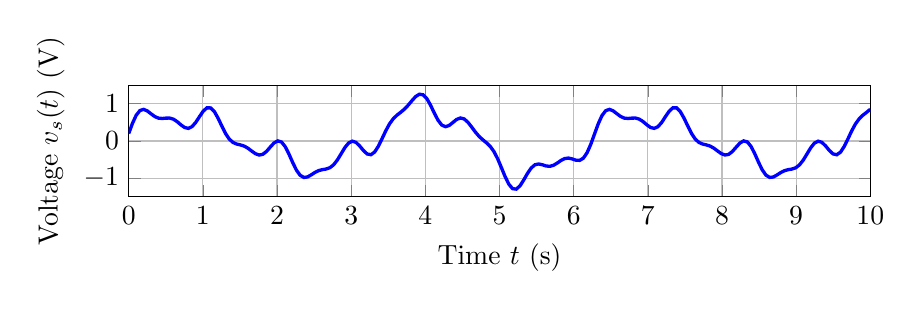
\begin{tikzpicture}
        \begin{axis}[
            width=11cm, height=3cm,
            xlabel={Time $t$ (s)},
            ylabel={Voltage $v_s(t)$ (V)},
            domain=0:10,
            samples=200,
            grid=major,
            xmin=0, xmax=10,
            ymin=-1.5, ymax=1.5,
        ]
        
        % Complex arbitrary waveform
        \addplot[blue, very thick] {
            0.8*sin(deg(2*x)) + 
            0.3*sin(deg(7*x)) + 
            0.15*sin(deg(13*x)) +
            0.2*cos(deg(3*x))
        };
        
        \end{axis}
    \end{tikzpicture}
    \vspace{-0.2cm}
    \caption{Example of an arbitrary voltage signal $v_s(t)$}
    \end{figure}
    
    % \vspace{0.4cm}
    
    \begin{columns}[t]
    \column{0.48\textwidth}
        \textbf{Characteristics}:
        \begin{itemize}
            \item Information in the ``warbles``
            \item Difficult to describe mathematically
        \end{itemize}
        
    \column{0.48\textwidth}
        \textbf{The Challenge}:
        \begin{itemize}
            \item How to process?
            \item How to design circuits?
        \end{itemize}
        
    \end{columns}
    
    % \vspace{0.3cm}
    
    \begin{block}{Solution}
        Frequency spectrum representation (Recall from Calculus: Fourier Series)
    \end{block}
    
\end{frame}

\section{Frequency Spectrum}

\begin{frame}{The Sinusoid:  Building Block of Signals}
    
    \begin{columns}[t]
    \column{0.5\textwidth}
        \textbf{Sine Wave Equation}:
        \[
        v_a(t) = V_a \sin(\omega t)
        \]
        
        \textbf{Parameters}:
        \begin{itemize}
            \item $V_a$: Peak amplitude (V)
            \item $\omega$: Angular frequency (rad/s)
            % \item $\omega = 2\pi f$
            \item $f = 1/T$: Frequency (Hz)
            \item $T$: Period (s)
        \end{itemize}
        
        % \vspace{0.3cm}
        
        \textbf{RMS Value}:
        \[
        V_{rms} = \frac{V_a}{\sqrt{2}}
        \]
        
        
    \column{0.48\textwidth}
        \begin{figure}[htb]
        \centering
        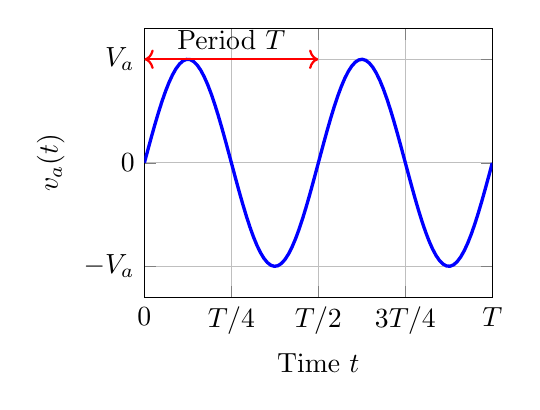
\begin{tikzpicture}
            \begin{axis}[
                width=6cm, height=5cm,
                xlabel={Time $t$},
                ylabel={$v_a(t)$},
                domain=0:4*pi,
                samples=100,
                grid=major,
                xmin=0, xmax=4*pi,
                ymin=-1.3, ymax=1.3,
                xtick={0, pi, 2*pi, 3*pi, 4*pi},
                xticklabels={0, $T/4$, $T/2$, $3T/4$, $T$},
                ytick={-1, 0, 1},
                yticklabels={$-V_a$, 0, $V_a$},
            ]
            
            \addplot[blue, very thick] {sin(deg(x))};
            
            % Period arrow
            \draw[<->, thick, red] (axis cs:0,1) -- (axis cs:2*pi,1);
            \node[above] at (axis cs:pi,1) {Period $T$};
            
            \end{axis}
        \end{tikzpicture}
        \caption{Sinusoidal voltage signal}
        \end{figure}
        
    \end{columns}
    
    \vspace{-0.4cm}
    
    \begin{block}{Key Concept}
        ANY signal can be represented as a sum of sinusoids 
    \end{block}
    
\end{frame}

\begin{frame}{Fourier Series:  Periodic Signals}
    
    \textbf{Concept}: Express periodic signals as sum of harmonically related sinusoids
    
    \vspace{0.3cm}
    
    \begin{columns}[t]
    \column{0.48\textwidth}
        \textbf{Square Wave Example}:
        
        \begin{figure}[htb]
        \centering
        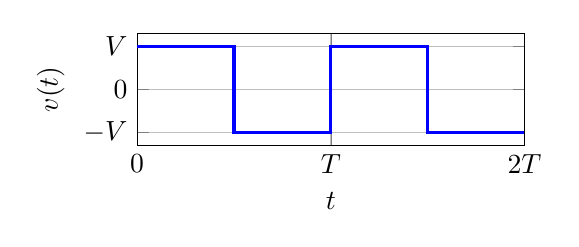
\begin{tikzpicture}
            \begin{axis}[
                width=6.5cm, height=3cm,
                xlabel={$t$},
                ylabel={$v(t)$},
                domain=0:4*pi,
                samples=500,
                grid=major,
                xmin=0, xmax=4*pi,
                ymin=-1.3, ymax=1.3,
                xtick={0, 2*pi, 4*pi},
                xticklabels={0, $T$, $2T$},
                ytick={-1, 0, 1},
                yticklabels={$-V$, 0, $V$},
            ]
            
            % Square wave
            \addplot[blue, very thick, const plot] coordinates {
                (0,1) (pi,1) (pi,-1) (2*pi,-1) (2*pi,1) (3*pi,1) (3*pi,-1) (4*pi,-1)
            };
            
            \end{axis}
        \end{tikzpicture}
        \caption{Symmetrical square wave}
        \end{figure}
        
        \vspace{-0.2cm}
        

        
    \column{0.48\textwidth}
        \textbf{Frequency Spectrum}: 
        
        \begin{figure}[htb]
        \centering
        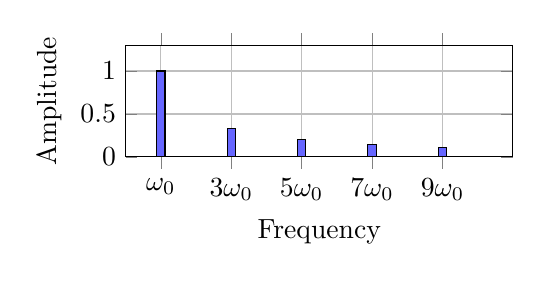
\begin{tikzpicture}
            \begin{axis}[
                width=6.5cm, height=3cm,
                xlabel={Frequency},
                ylabel={Amplitude},
                ybar,
                bar width=3pt,
                xmin=0, xmax=11,
                ymin=0, ymax=1.3,
                xtick={1,3,5,7,9},
                xticklabels={$\omega_0$, $3\omega_0$, $5\omega_0$, $7\omega_0$, $9\omega_0$},
                grid=major,
                ylabel style={align=center},
            ]
            
            \addplot[fill=blue! 60] coordinates {
                (1, 1.0) (3, 0.333) (5, 0.2) (7, 0.143) (9, 0.111)
            };
            
            \end{axis}
        \end{tikzpicture}
        \caption{Line spectrum of square wave}
        \end{figure}
        
    \end{columns}

    \textbf{Fourier Series}:
    \[
    v(t) = \frac{4V}{\pi}\left(\sin\omega_0 t + \frac{1}{3}\sin 3\omega_0 t + \frac{1}{5}\sin 5\omega_0 t + \cdots\right), \text{ where }  \omega_0 = \frac{2\pi}{T} \text{ is the fund. freq.}
    \]
    

    
\end{frame}

\begin{frame}{Building a Square Wave from Sinusoids}
    
    \begin{figure}[htb]
    \centering
    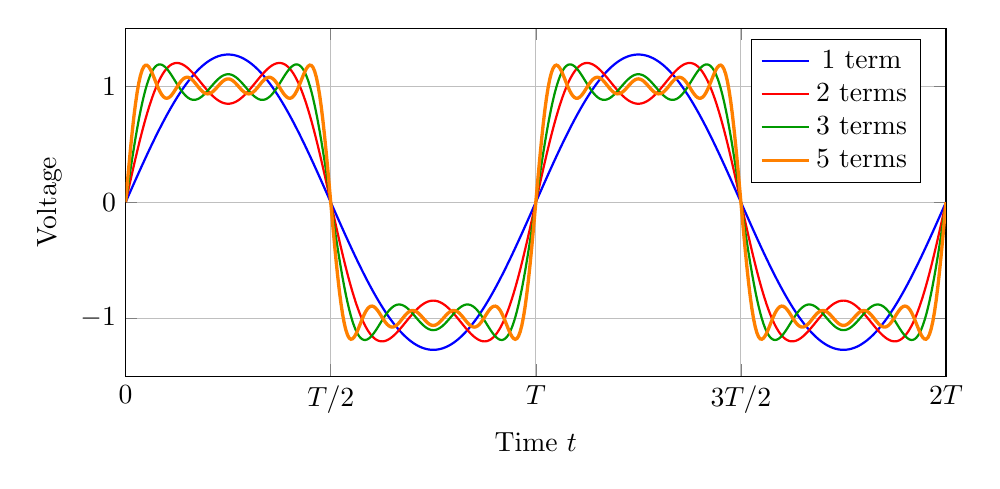
\begin{tikzpicture}
        \begin{axis}[
            width=12cm, height=6cm,
            xlabel={Time $t$},
            ylabel={Voltage},
            domain=0:4*pi,
            samples=500,
            grid=major,
            xmin=0, xmax=4*pi,
            ymin=-1.5, ymax=1.5,
            legend pos=north east,
            xtick={0, pi, 2*pi, 3*pi, 4*pi},
            xticklabels={0, $T/2$, $T$, $3T/2$, $2T$},
        ]
        
        % Fundamental only
        \addplot[blue, thick] {(4/pi)*sin(deg(x))};
        \addlegendentry{1 term}
        
        % Fundamental + 3rd harmonic
        \addplot[red, thick] {(4/pi)*(sin(deg(x)) + (1/3)*sin(deg(3*x)))};
        \addlegendentry{2 terms}
        
        % Up to 5th harmonic
        \addplot[green!60! black, thick] {(4/pi)*(sin(deg(x)) + (1/3)*sin(deg(3*x)) + (1/5)*sin(deg(5*x)))};
        \addlegendentry{3 terms}
        
        % Up to 9th harmonic
        \addplot[orange, very thick] {(4/pi)*(sin(deg(x)) + (1/3)*sin(deg(3*x)) + (1/5)*sin(deg(5*x)) + (1/7)*sin(deg(7*x)) + (1/9)*sin(deg(9*x)))};
        \addlegendentry{5 terms}
        
        \end{axis}
    \end{tikzpicture}
    \caption{Fourier series approximation improves with more terms}
    \end{figure}
    
\end{frame}

\begin{frame}{Fourier Transform: Nonperiodic Signals}
  \textbf{For Nonperiodic Signals}:
  \begin{itemize}
    \item Fourier Transform (not series)
    \item \textbf{Continuous} frequency spectrum
    \item Contains all frequencies
    \item Notation: $v_a(t) \leftrightarrow V_a(\omega)$
  \end{itemize}

  \begin{columns}[t]
    \column{0.48\textwidth}
      {\centering
      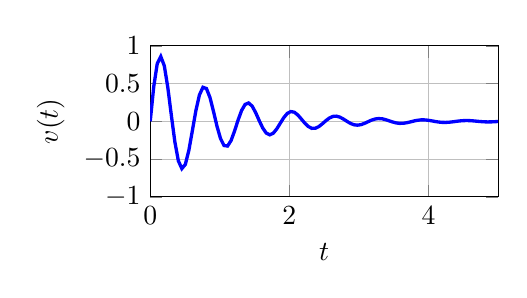
\begin{tikzpicture}
        \begin{axis}[
          width=6cm, height=3.5cm,
          xlabel={$t$}, ylabel={$v(t)$},
          domain=0:5, samples=100,
          grid=major,
          xmin=0, xmax=5,
          ymin=-1.0, ymax=1.0,
          xtick={}, ytick={},
        ]
          \addplot[blue, very thick] {exp(-x)*sin(deg(10*x))};
        \end{axis}
      \end{tikzpicture}
      \captionof{figure}{Nonperiodic signal}\par
      }

    \column{0.48\textwidth}
      {\centering
      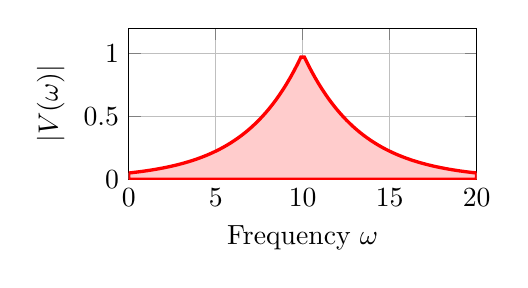
\begin{tikzpicture}
        \begin{axis}[
          width=6cm, height=3.5cm,
          xlabel={Frequency $\omega$}, ylabel={$|V(\omega)|$},
          domain=0:20, samples=100,
          grid=major,
          xmin=0, xmax=20,
          ymin=0, ymax=1.2,
          xtick={}, ytick={},
        ]
          \addplot[red, very thick, fill=red!20] {exp(-0.3*abs(x-10))} \closedcycle;
        \end{axis}
      \end{tikzpicture}
      \captionof{figure}{Continuous frequency spectrum}\par
      }
  \end{columns}
\end{frame}

\begin{frame}{Time vs.  Frequency Domain}
    
    \begin{columns}[t]
    \column{0.48\textwidth}
        \textbf{Time Domain}:
        \begin{itemize}
            \item Signal as $v(t)$ vs. time
            \item Shows temporal behavior
            \item Direct measurement
            \item Oscilloscope view
        \end{itemize}
        
        \vspace{0.3cm}
        
        \begin{figure}[htb]
        \centering
        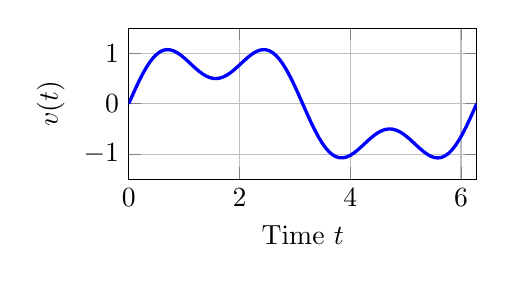
\begin{tikzpicture}
            \begin{axis}[
                width=6cm, height=3.5cm,
                xlabel={Time $t$},
                ylabel={$v(t)$},
                domain=0:2*pi,
                samples=100,
                grid=major,
                xmin=0, xmax=2*pi,
                ymin=-1.5, ymax=1.5,
                xtick={},
                ytick={},
            ]
            
            \addplot[blue, very thick] {sin(deg(x)) + 0.5*sin(deg(3*x))};
            
            \end{axis}
        \end{tikzpicture}
        \caption{Time-domain representation}
        \end{figure}
        
    \column{0.48\textwidth}
        \textbf{Frequency Domain}:
        \begin{itemize}
            \item Signal as $V(\omega)$ vs. frequency
            \item Shows frequency content
            \item Reveals hidden components
            \item Spectrum analyzer view
        \end{itemize}
        
        % \vspace{0.3cm}
        
        \begin{figure}[htb]
        \centering
        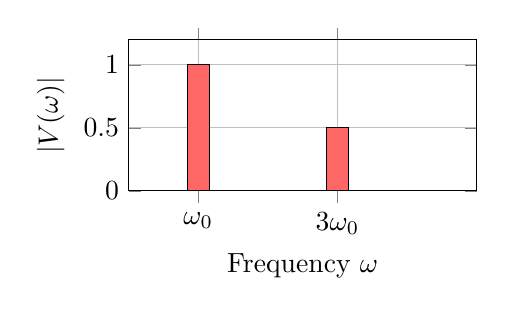
\begin{tikzpicture}
            \begin{axis}[
                width=6cm, height=3.5cm,
                xlabel={Frequency $\omega$},
                ylabel={$|V(\omega)|$},
                ybar,
                bar width=8pt,
                xmin=0, xmax=5,
                ymin=0, ymax=1.2,
                xtick={1,3},
                xticklabels={$\omega_0$, $3\omega_0$},
                grid=major,
            ]
            
            \addplot[fill=red!60] coordinates {(1,1.0) (3,0.5)};
            
            \end{axis}
        \end{tikzpicture}
        \caption{Frequency-domain representation}
        \end{figure}
        
    \end{columns}
    
    \vspace{0.3cm}
    
    \begin{block}{Two Views of the Same Signal}
        $v_a(t)$ (time domain) $\longleftrightarrow$ $V_a(\omega)$ (frequency domain)
    \end{block}
    
\end{frame}

\section{Summary}

\begin{frame}{Summary}
    
    \begin{columns}[t]
    \column{0.48\textwidth}

        
        \textbf{Signals}:
        \begin{itemize}
            \item Carry information
            \item Transducers convert to electrical
            \item Represented as voltage or current
        \end{itemize}
        
        \vspace{0.3cm}
        
        \textbf{Signal Sources}:
        \begin{itemize}
            \item Thevenin:  voltage + $R_s$
            \item Norton: current + $R_s$
            \item Source resistance limits delivery
        \end{itemize}
        
    \column{0.48\textwidth}
        \textbf{Frequency Spectrum}:
        \begin{itemize}
            \item Signals as sum of sinusoids
            \item Fourier series: periodic signals
            \item Fourier transform: nonperiodic
            \item Line vs. continuous spectra
        \end{itemize}
        
        \vspace{0.3cm}
        
        \textbf{Two Representations}:
        \begin{itemize}
            \item Time domain: $v(t)$
            \item Frequency domain:  $V(\omega)$
        \end{itemize}
        
    \end{columns}
    
    \vspace{0.4cm}
    
\end{frame}

\end{document}